\newcommand{\econtexRoot}{Paper/}
% The \commands below are required to allow sharing of the same base code via Github between TeXLive on a local machine and ShareLaTeX.  This is an ugly solution to the requirement that custom LaTeX packages be accessible, and that ShareLaTeX seems to ignore symbolic links (even if they are relative links to valid locations)
\providecommand{\econtex}{\econtexRoot/texmf-local/tex/latex/econtex}
\providecommand{\econtexSetup}{\econtexRoot/texmf-local/tex/latex/econtexSetup}
\providecommand{\econtexShortcuts}{\econtexRoot/texmf-local/tex/latex/econtexShortcuts}
\providecommand{\econtexBibMake}{\econtexRoot/texmf-local/tex/latex/econtexBibMake}
\providecommand{\econtexBibStyle}{\econtexRoot/texmf-local/bibtex/bst/econtex}
\providecommand{\notes}{\econtexRoot/texmf-local/tex/latex/handout}
\providecommand{\handoutSetup}{\econtexRoot/texmf-local/tex/latex/handoutSetup}
\providecommand{\handoutShortcuts}{\econtexRoot/texmf-local/tex/latex/handoutShortcuts}
\providecommand{\handoutBibMake}{\econtexRoot/texmf-local/tex/latex/handoutBibMake}
\providecommand{\handoutBibStyle}{\econtexRoot/texmf-local/bibtex/bst/handout}

  

\documentclass{beamer}
\usepackage{etoolbox}
\usepackage{comment}
\usepackage{graphicx}
%\usepackage{dtklogos}
\usepackage{dsfont}
\usepackage{amsmath,amssymb}
\usepackage{\econtexShortcuts}
\usepackage[english]{babel}
\usepackage[svgnames,hyperref]{}
\usepackage{empheq}
\usepackage[many]{tcolorbox}
\usepackage{remreset}
\usepackage{tikz} 
\usetikzlibrary{tikzmark,fit,shapes.geometric}
\usetikzlibrary{tikzmark,calc,arrows,shapes,decorations.pathreplacing}
\tikzset{every picture/.style={remember picture}}
\usepackage{cancel}
\usepackage{booktabs,natbib}
\setbeamercovered{invisible}

\usepackage{dcolumn}

\tcbset{highlight math style={enhanced,
		colframe=red!60!black,colback=yellow!50!white,arc=4pt,boxrule=1pt,
}}


\makeatletter
\@removefromreset{subsection}{section}
\patchcmd{\beamer@part}{\setcounter{subsection}{0}}{}{}
\makeatother
\setcounter{subsection}{1}
\setbeamercovered{transparent}
\setbeamertemplate{navigation symbols}{}%remove navigation symbols
\begin{comment}
\setbeamertemplate{footline}
{
	\hbox{\begin{beamercolorbox}[wd=1\paperwidth,ht=2.25ex,dp=1ex,right]{framenumber}%
			\usebeamerfont{framenumber}\insertframenumber{} \hspace*{2ex}
	\end{beamercolorbox}}%
	\vskip0pt%
}
\end{comment}


\mode<presentation>{}
%% preamble
\title[Consumption Heterogeneity: Micro Drivers and Macro Implications]{Consumption Heterogeneity: \\ Micro Drivers and Macro Implications}
\author{Edmund Crawley \hspace{0.7cm} Andreas Kuchler \textcolor{white}{..} }
\institute{Federal Reserve Board \hspace{0.7cm} Danmarks Nationalbank  \vspace{0.5cm}}
%\date[08/11/2018]{Towson University\\ November 8, 2018}
\date[12/12/2019]{CFPB Research Conference \\ December 12, 2019 \vspace{2cm} \\ \footnotesize Viewpoints and conclusions stated in this paper are the responsibility of the authors alone and do not necessarily reflect the viewpoints of the Federal Reserve Board or Danmarks Nationalbank.}
\usetheme{Frankfurt}
\setbeamertemplate{navigation symbols}{}
\makeatletter
\setbeamertemplate{footline}
{%
	\hbox{\begin{beamercolorbox}[wd=1\paperwidth,ht=2.25ex,dp=1ex,right]{framenumber}%
		\usebeamerfont{framenumber}\insertframenumber{} \hspace*{2ex}
	\end{beamercolorbox}}%
	\vskip0pt%
	\pgfuseshading{beamer@barshade}%
	\ifbeamer@sb@subsection%
	\vskip-9.75ex%
	\else%
	\vskip-7ex%
	\fi%
	\begin{beamercolorbox}[ignorebg,ht=2.25ex,dp=3.75ex]{section in head/foot}
		\insertnavigation{\paperwidth}
	\end{beamercolorbox}%
	\ifbeamer@sb@subsection%
	\begin{beamercolorbox}[ignorebg,ht=2.125ex,dp=1.125ex,%
		leftskip=.3cm,rightskip=.3cm plus1fil]{subsection in head/foot}
		\usebeamerfont{subsection in head/foot}\insertsubsectionhead \insertframenumber{} \hspace*{2ex}
	\end{beamercolorbox}%
	\fi%
}%
\setbeamertemplate{headline}{%
}
\makeatother
\begin{document}
\setbeamertemplate{caption}{\raggedright\insertcaption\par}
\newcolumntype{d}[1]{D{.}{.}{#1}}
%circled draws a circle around a number
\newcommand*\circled[1]{\tikz[baseline=(char.base)]{
		\node[shape=circle,draw,inner sep=2pt] (char) {#1};}}

\begin{frame}[plain]
\titlepage
\end{frame}
\addtocounter{framenumber}{-1}
\section{Introduction}
\setbeamercovered{invisible}
\frame
{
	\frametitle{What Do We Do?}
	\begin{center}
	We estimate the \textbf{consumption response} \\
	\bigskip
	 to permanent and transitory \textbf{shocks to income} \\
	 \bigskip
	 for \textbf{different groups} of households
	 \end{center}
}
\frame[t]
{
	\frametitle{Hasn't This Been Done Before?}
	\vspace{1.8cm}
	Yes, but...\\
	\bigskip
	\hspace{1cm} Our \textbf{method} addresses bias in previous results  \tikz[baseline]{\node(bias){}}\\
	\bigskip
	\hspace{1cm} Our \textbf{data} allows sharp focus on household heterogeneity  \tikz[baseline]{\node(data){}}\\ 
	\only<2->{
	\begin{tikzpicture}[remember picture,overlay]
	\node (bias1a)  at ([shift={(-3.5,0.3)}]bias) {};
	\node (bias1b)  at ([shift={(0,1)}]bias1a) {};
	\draw[blue,thick,->] (bias1a)  to [in=270,out=90] (bias1b) node[anchor=south,text = blue] {Time Aggregation Problem};
	\end{tikzpicture}
	}
	\only<3->{
	\begin{tikzpicture}[remember picture,overlay]
	\node (data1a)  at ([shift={(-8.2,-0.0)}]data) {};
	\node (data1b)  at ([shift={(0.5,-1)}]data1a) {};
	\draw[blue,thick,->] (data1a)  to [in=180,out=270] (data1b) node[anchor=west,text = blue] {\begin{tabular}{l} Sample size in millions\\ Detailed balance sheet \end{tabular}};
	\end{tikzpicture}
	}
}
\begin{comment}
\frame
{
	\frametitle{Why Do We Care? (as macroeconomists)}
	1) Heterogenous agent models have testable micro behavior \tikz[baseline]{\node(micro){}}\\
	\bigskip
	2) Quantify Macro Implications \tikz[baseline]{\node(macro){}}
	\only<2->{
	\begin{tikzpicture}[remember picture,overlay]
	\node (micro1a)  at ([shift={(-2.2,0.3)}]micro) {};
	\node (micro1b)  at ([shift={(-1,0.8)}]micro1a) {};
	\draw[blue,thick,->] (micro1a)  to [in=270,out=90] (micro1b) node[anchor=south,text = blue] {\begin{tabular}{l} e.g. Consumption smoothing requires liquid wealth  \end{tabular}};
	\end{tikzpicture}
	}
	\only<3->{
	\begin{tikzpicture}[remember picture,overlay]
	\node (macro1a)  at ([shift={(-2.8,0.0)}]macro) {};
	\node (macro1b)  at ([shift={(-0.0,-0.8)}]macro1a) {};
	\draw[blue,thick,->] (macro1a)  to [in=90,out=270] (macro1b) node[anchor=north,text = blue] {\begin{tabular}{l} e.g. Redistribution in Monetary Policy  \end{tabular}};
	\end{tikzpicture}
	}
}
\end{comment}
\frame
{
	\frametitle{What do we find? (Liquid Wealth)}
	Low Liquid Wealth Households:
	\begin{itemize}
		\item Hand-to-Mouth
		\item Spend 85 cents out of every marginal dollar, both transitory and permanent
	\end{itemize}
	\bigskip
	\pause
	High Liquid Wealth Households: 
	\begin{itemize}
		\item Large Response to Transitory Shocks (25 cents per dollar)
		\item Small Response to Permanent Shocks (60 cents per dollar)
	\end{itemize}
	relative to Permanent Income Hypothesis or Buffer-Stock models
}
\frame[t]
{
	\frametitle{What do we find? (Redistribution in Monetary Policy)}
	\only<1>{
		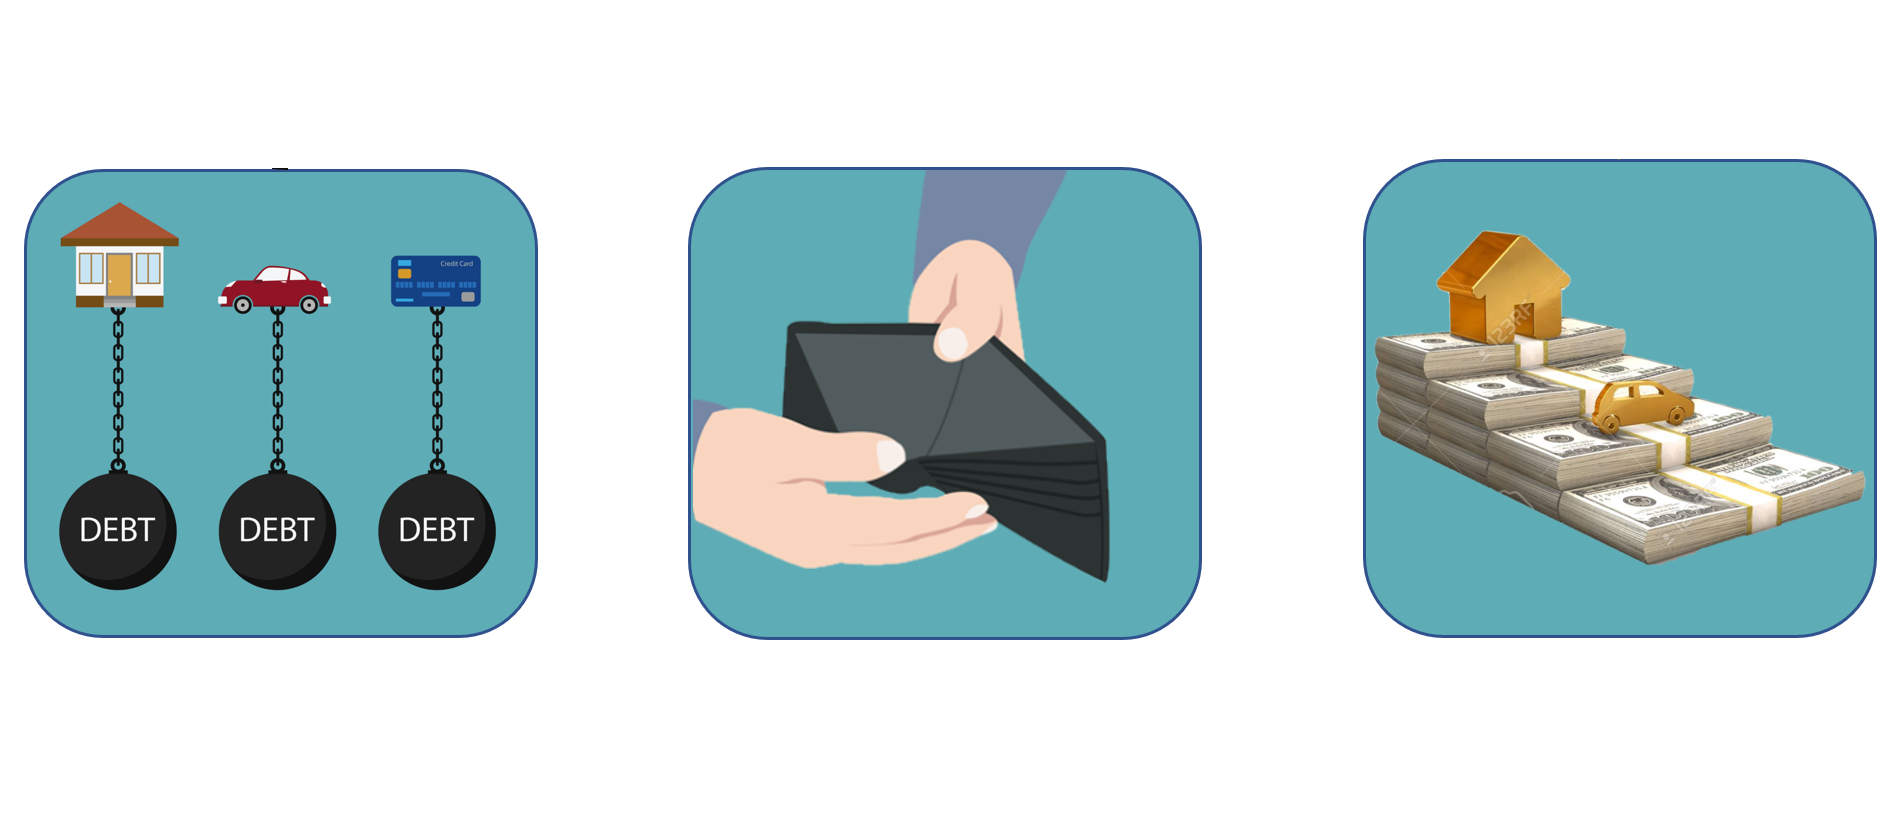
\includegraphics[width=11cm]{./SlideFigures/IRE_Big1.png}
	}
	\only<2>{
	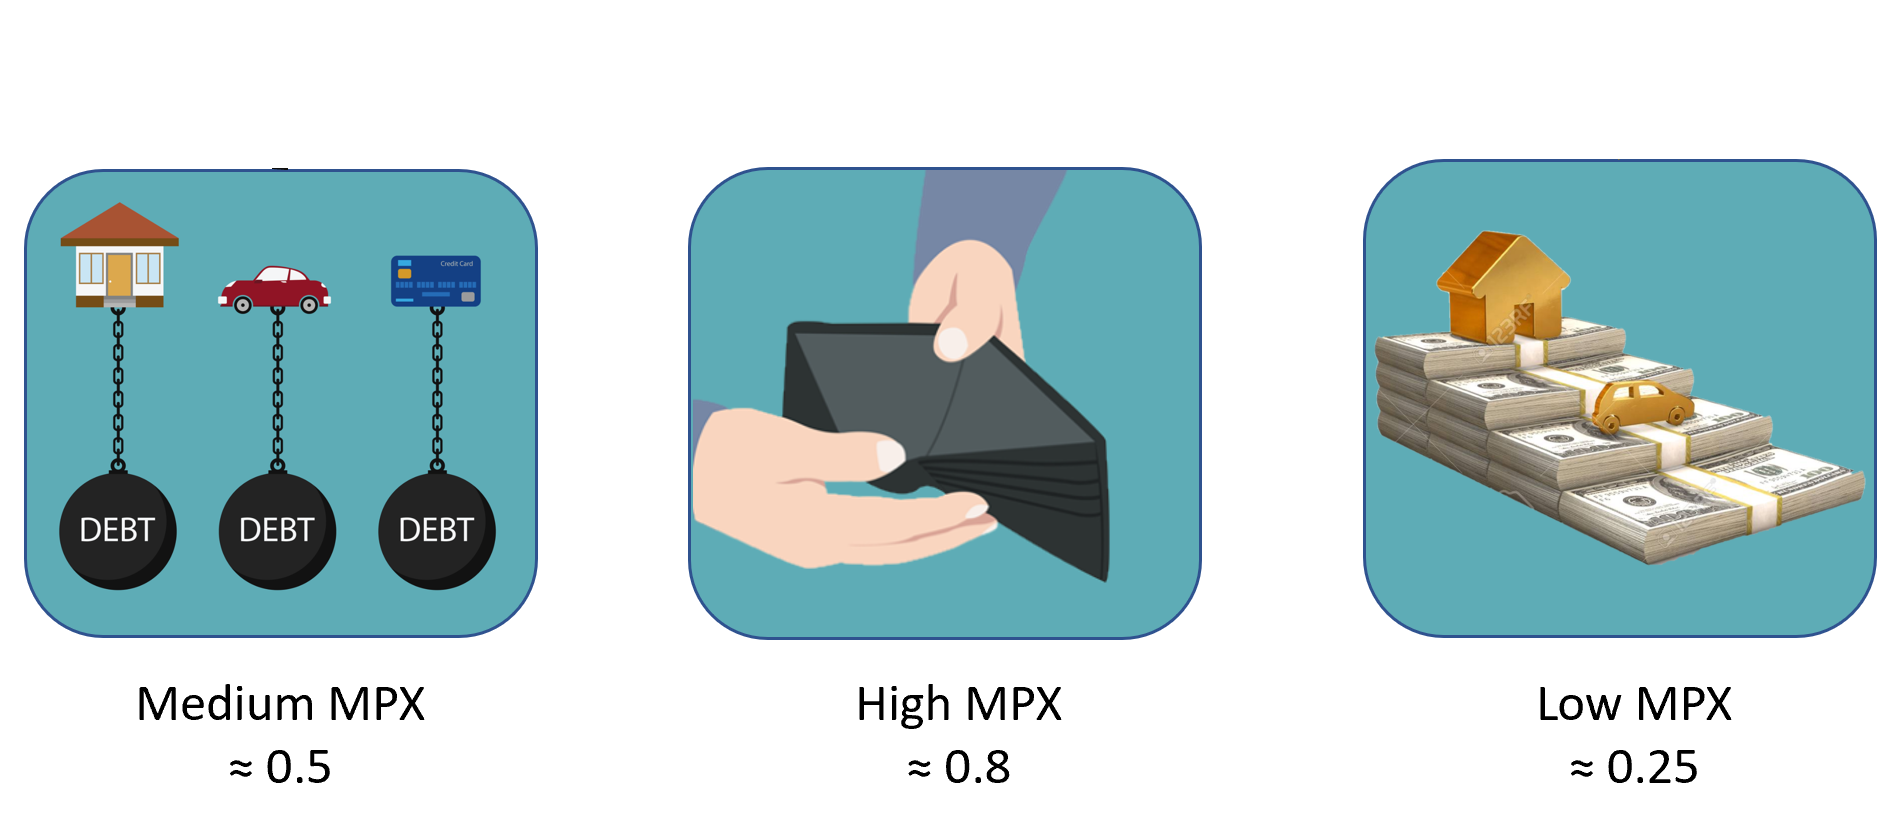
\includegraphics[width=11cm]{./SlideFigures/IRE_Big2.png}
	\\[0.7cm]
	MPX: Marginal Propensity to eXpend (includes durables)
	}
	\only<3->{
	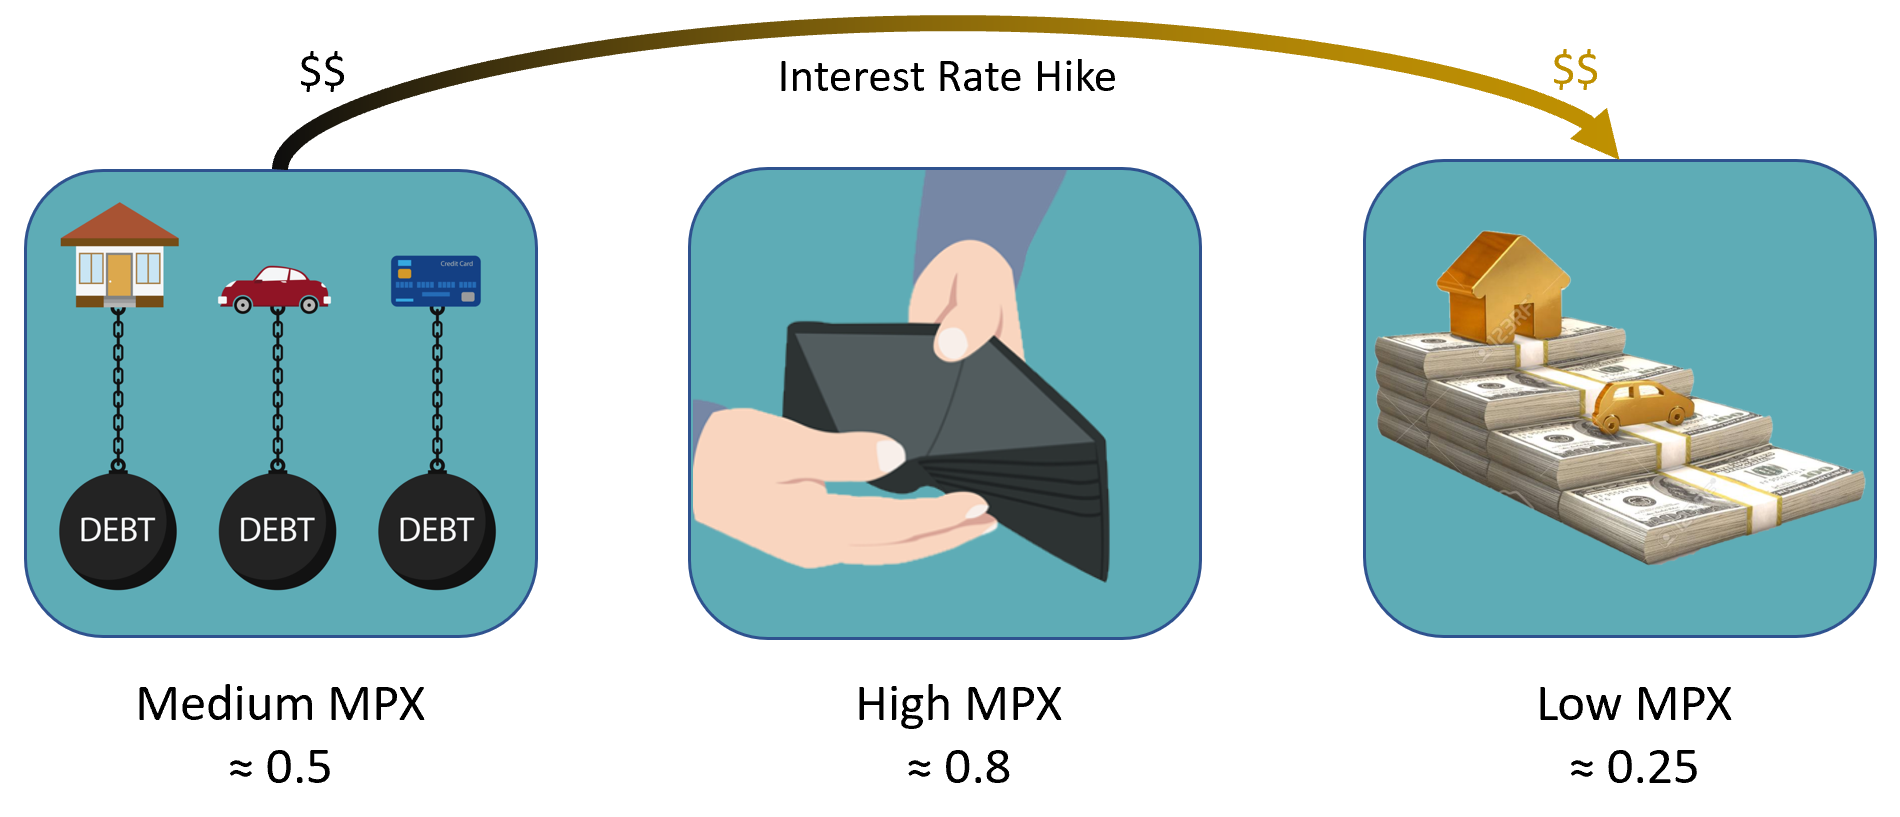
\includegraphics[width=11cm]{./SlideFigures/IRE_Big3.png} \tikz[baseline]{\node(ire){}}
	}
	\only<3>{
	\begin{tikzpicture}[remember picture,overlay]
	\node (ire1a)  at ([shift={(1.3,0.3)}]ire) {};
	\node (ire1b)  at ([shift={(-0.4,-0.4)}]ire1a) {};
	\draw[blue,thick,->] (ire1a)  to [in=45,out=225] (ire1b) node[anchor=north,text = blue] {\begin{tabular}{l} Decrease spending \\ a \textit{lot}  \end{tabular}};
	\node (ire1c)  at ([shift={(9.5,0.3)}]ire) {};
	\node (ire1d)  at ([shift={(0.4,-0.4)}]ire1c) {};
	\draw[blue,thick,->] (ire1c)  to [in=135,out=315] (ire1d) node[anchor=north,text = blue] {\begin{tabular}{r} Increase spending \\ a \textit{little}  \end{tabular}};
	\end{tikzpicture}
	}
	\only<4->{
	\vspace{-.5cm}
	\begin{align*}
	\text{1yr rate }&\uparrow \ 1\% \\
	\tikz[baseline]{\node(aggregate){}} \textit{Aggregate}\text{ Spending }&\downarrow \ 26 \text{ basis points}
	\end{align*}
	\begin{tikzpicture}[remember picture,overlay]
	\node (aggregatea)  at ([shift={(1.5,-0.1)}]aggregate) {};
	\node (aggregateb)  at ([shift={(-0.4,-0.4)}]aggregatea) {};
	\draw[blue,thick,->] (aggregatea)  to [in=45,out=225] (aggregateb) node[anchor=north,text = blue] {Through this redistribution channel \textit{alone}};
	\end{tikzpicture}
	}
}
\section{Empirical Strategy}
\setbeamercovered{invisible}
\frame[t]{
	\frametitle{How Do We Do This? Reduced Form Approach}
	Identifying Restrictions on\\
	\bigskip
	\hspace{1cm}\textbf{Income}\tikz[baseline]{\node(income){}}\\
	\bigskip
	\hspace{1cm}and\\
	\bigskip
	\hspace{1cm}\textbf{Consumption}\tikz[baseline]{\node(consumption){}}\\
	\bigskip
	In \textbf{Continuous} Time\tikz[baseline]{\node(continuous){}}\\
	\vspace{0.8cm}
	\only<2->{
	\begin{tikzpicture}[remember picture,overlay]
	\node (incomea)  at ([shift={(0,0.1)}]income) {};
	\node (incomeb)  at ([shift={(1.5,0)}]incomea) {};
	\node (incomebshiftback)  at ([shift={(1.2,0)}]incomea) {};
	\node (incomec)  at ([shift={(2,0)}]incomea) {};
	\node (incomecup)  at ([shift={(2,0.2)}]incomea) {};
	\node (incomecdown)  at ([shift={(2,-0.2)}]incomea) {};
	\node (consumptiona)  at ([shift={(0,0.1)}]consumption) {};
	\node (consumptionb)  at ([shift={(0.5,0)}]consumptiona) {};
	\node (consumptionbshiftback)  at ([shift={(0.2,0)}]consumptiona) {};
	\node (consumptionc)  at ([shift={(1,0)}]consumptiona) {};
	\node (consumptioncup)  at ([shift={(1,0.2)}]consumptiona) {};
	\node (consumptioncdown)  at ([shift={(1,-0.2)}]consumptiona) {};
	\draw[white,thick,->] (incomea)  to [in=180,out=0] (incomec) node[anchor=west,text = blue] {\begin{tabular}{lcl}  Permanent & (random walk) & shocks\\ Transitory & ($<$2 years) & shocks  \end{tabular}};
	\draw[blue,thick,-] (incomea)  to [in=180,out=0] (incomeb) {};
	\draw[blue,thick,->] (incomebshiftback)  to [in=180,out=0] (incomecup) {};
	\draw[blue,thick,->] (incomebshiftback)  to [in=180,out=0] (incomecdown) {};
		\end{tikzpicture}
	}
	\only<3->{
	\begin{tikzpicture}[remember picture,overlay]
	\draw[white,thick,->] (consumptiona)  to [in=180,out=0] (consumptionc) node[anchor=west,text = blue] {\begin{tabular}{lcl}  Permanent & (random walk) & response\\ Transitory & ($<$2 years) & response  \end{tabular}};
	\draw[blue,thick,-] (consumptiona)  to [in=180,out=0] (consumptionb) {};
	\draw[blue,thick,->] (consumptionbshiftback)  to [in=180,out=0] (consumptioncup) {};
	\draw[blue,thick,->] (consumptionbshiftback)  to [in=180,out=0] (consumptioncdown) {};
	\end{tikzpicture}
	}
	\only<4->{
	\begin{tikzpicture}[remember picture,overlay]
	\node (continuousa)  at ([shift={(0,0.1)}]continuous) {};
	\node (continuousb)  at ([shift={(1,0)}]continuousa) {};
	\draw[blue,thick,->] (continuousa)  to [in=180,out=0] (continuousb) node[anchor=west,text = blue] {\begin{tabular}{lcl} Time Aggregation Problem  \end{tabular}};
	\end{tikzpicture}
	}
}
\frame
{
	\frametitle{Identification Restrictions: Income Process}
	\begin{itemize} 
		\item Permanent Income (random walk)
		\item Transitory Income (persistence $<$ 2 years)
	\end{itemize}
\vspace{-0.2cm}
	\begin{figure}
		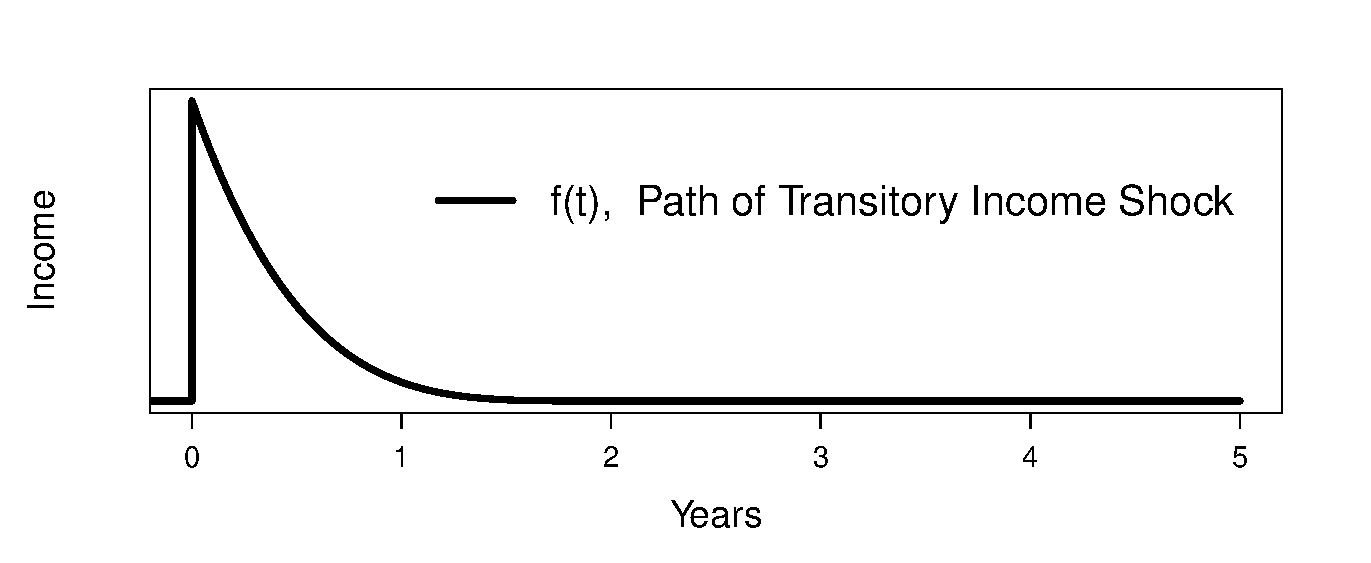
\includegraphics[scale=0.35,trim= 0 0.6cm 0 1.2cm,clip]{../Figures/GenericTransitory_slides.pdf}
	\end{figure}
	\vspace{-0.5cm}
	\begin{align*}
	\onslide<2->{\onslide<3->{\color{blue} \tikz[baseline]{\node(n1){}}\bar{y}_T =} \onslide<3->{\tikz[baseline]{\node(n2){}}\int_{T-1}^{T}}\color{black} y_t\onslide<3->{\color{blue}dt} &= \onslide<3->{ \color{blue} \int_{T-1}^{T}}\color{black} \tikz[baseline]{\node(n4){}}p_t \onslide<3->{\color{blue}dt} \color{black} + \onslide<3->{\color{blue}\int_{T-1}^{T}}\color{black}\int_{t-2}^{t} \tikz[baseline]{\node(n5){}}f(t-s)dq_s\onslide<3->{\color{blue}dt}  }
	\end{align*}
	\only<2>{
	\begin{tikzpicture}[remember picture,overlay]
	\node (n4a)  at ([shift={(0.2,-0.05)}]n4) {};
	\node (n5a)  at ([shift={(0.5,-0.2)}]n5) {};
	\draw[blue,thick,->] (n4a)  to [in=90,out=245] + (225:1.3cm) node[anchor=north,text = blue] {Permanent income flow};
	\draw[blue,thick,->] (n5a) to [in=90,out=245] + (290:0.8cm) node[anchor=north,text = blue] {Transitory income flow};
	\end{tikzpicture}
	}
	\only<3>{
	\begin{tikzpicture}[remember picture,overlay]
	\node (n1a)  at ([shift={(0.25,0.2)}]n1) {};
	\node (n2a)  at ([shift={(0.45,-0.45)}]n2) {};
	\draw[blue,thick,->] (n1a)  to [in=270,out=90] + (90:0.6cm) node[anchor=south,text = blue] {Observed Income};
	\draw[blue,thick,->] (n2a)  to [in=90,out=270] + (270:0.6cm) node[anchor=north,text = blue] {Time Aggregation};
	\end{tikzpicture}
	}
}
\frame
{
	\frametitle{Identification Restrictions: Consumption Response}
	\label{cons_identification}
	\begin{itemize}
		\item Permanent: Moves by fraction $\phi$ of shock
		\item Transitory: Persistence $<$ 2 years \qquad \qquad \qquad \qquad \hyperlink{cons_decay}{\beamerbutton{Evidence}}
	\end{itemize}
\vspace{-0.2cm}
	\begin{figure}
	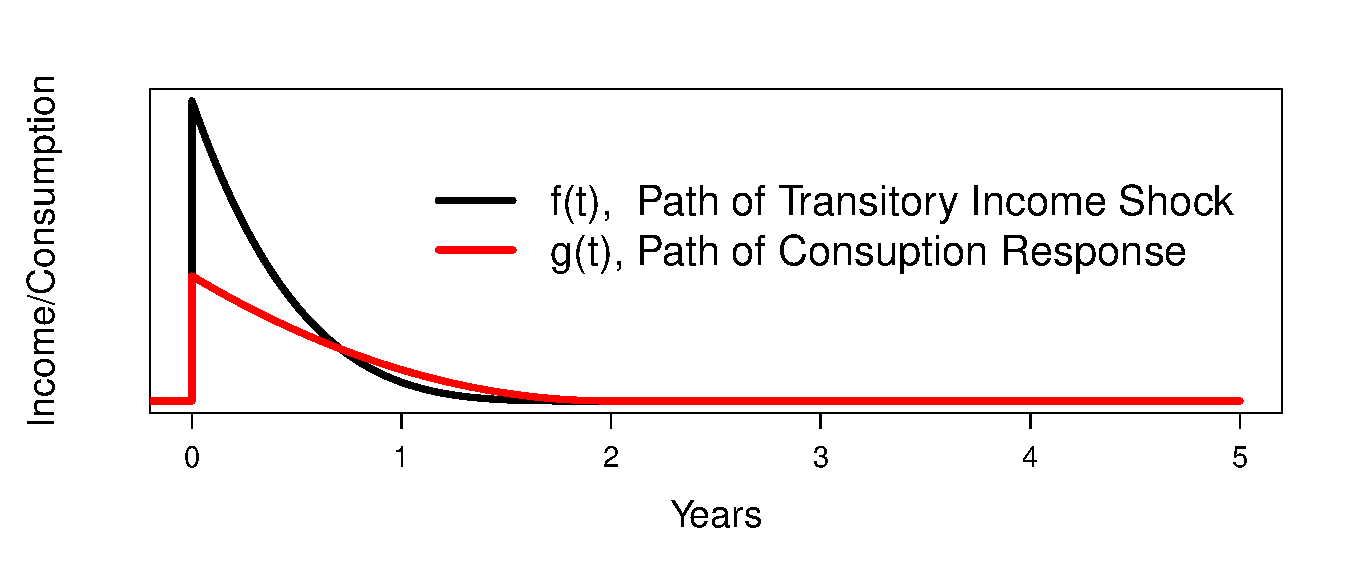
\includegraphics[scale=0.35,trim= 0 0.6cm 0 1.2cm,clip]{../Figures/GenericTransitoryConsumption_slides.pdf}
\end{figure}
\vspace{-0.5cm}
\begin{align*}
\onslide<2->{\onslide<3->{\color{blue} \tikz[baseline]{\node(n1){}}\bar{c}_T =} \onslide<3->{\tikz[baseline]{\node(n2){}}\int_{T-1}^{T}}\color{black} c_t\onslide<3->{\color{blue}dt} &= \onslide<3->{ \color{blue} \int_{T-1}^{T}}\color{black} \tikz[baseline]{\node(n4){}}\phi p_t \onslide<3->{\color{blue}dt} \color{black} + \onslide<3->{\color{blue}\int_{T-1}^{T}}\color{black}\int_{t-2}^{t} \tikz[baseline]{\node(n5){}}g(t-s)dq_s\onslide<3->{\color{blue}dt}}
\end{align*}
\only<2>{
	\begin{tikzpicture}[remember picture,overlay]
	\node (n4a)  at ([shift={(0.2,-0.05)}]n4) {};
	\node (n5a)  at ([shift={(0.5,-0.2)}]n5) {};
	\draw[blue,thick,->] (n4a)  to [in=90,out=245] + (225:1.3cm) node[anchor=north,text = blue] {Permanent consumption flow};
	\draw[blue,thick,->] (n5a) to [in=90,out=245] + (290:0.8cm) node[anchor=north,text = blue] {Transitory consumption flow};
	\end{tikzpicture}
}
\only<3>{
	\begin{tikzpicture}[remember picture,overlay]
	\node (n1a)  at ([shift={(0.25,0.2)}]n1) {};
	\node (n2a)  at ([shift={(0.45,-0.45)}]n2) {};
	\draw[blue,thick,->] (n1a)  to [in=270,out=90] + (90:0.6cm) node[anchor=south,text = blue] {h \ \ \ \ \ \ Observed Consumption};
	\draw[blue,thick,->] (n2a)  to [in=90,out=270] + (270:0.6cm) node[anchor=north,text = blue] {Time Aggregation};
	\end{tikzpicture}
}
}
\frame
{
	\frametitle{Full Identification}
We use GMM on the equations:
\begin{empheq}[box=\tcbhighmath]{align*}
\mathrm{Var}(\Delta^N \bar{y_T} ) &= \hspace{0.55em} \Big(N-\frac{1}{3}\Big) \sigma^2_p + 2  \sigma^2_{\tilde{q}} \\
\mathrm{Cov}(\Delta^N \bar{c_T},\Delta^N \bar{y_T} ) &= \phi \Big(N-\frac{1}{3}\Big) \sigma^2_p + 2 \psi \sigma^2_{\tilde{q}}
\end{empheq}
with $N=3,4,5$ (and $T=2007,..,2015$) to identify:\\
\bigskip
\begin{itemize}
	\item $\sigma^2_p$: Permanent shock variance
	\item $\sigma^2_{\tilde{q}}$: (Time aggregated) transitory shock variance
	\item $\phi$: MPX out of permanent income shocks
	\item $\psi$: MPX out of transitory income shocks
\end{itemize}
\bigskip
where  $\psi$ is the regression coefficient of `transitory' consumption on transitory income
}
\section{Data}
\frame
{
	\label{data}
	\frametitle{Data}
	What we need:
	\begin{itemize}
		\item Panel Data on \textbf{Income} and \textbf{Expenditure}
		\item Household \textbf{Balance Sheets} 
	\end{itemize}
	\bigskip
	\pause
	What we have: Registry data for all Danish households
	\begin{itemize}
		\item \textbf{Income}
		\begin{itemize}
			\item[] Third party reported
			\item[] After-tax, restrict to heads aged 30-55
		\end{itemize}
		\item \textbf{Balance Sheet}
		\begin{itemize}
			\item[] Wealth on 31 Dec
			\item[] Asset category, mortgage tenure \hspace{1.5cm} 
		\end{itemize}
	\item \textbf{Expenditure}
		\begin{itemize}
		\item[] No \textit{direct} measure of spending
		\end{itemize}
	\end{itemize}
}
\frame[t]
{
	\frametitle{Data: Expenditure}
	\label{data_expenditure}
	Household budget constraint
		\begin{align*}
			\text{Expenditure} \qquad = \qquad \tikz[baseline]{\node(income){}}\text{Income}\qquad  - \qquad \tikz[baseline]{\node(saving){}}\text{Saving}
		\end{align*}
		\bigskip
	\only<2->{
	\begin{tikzpicture}[remember picture,overlay]
	\node (incomea)  at ([shift={(0.6,-0.1)}]income) {};
	\node (incomeb)  at ([shift={(0,-0.4)}]incomea) {};
	\node (savinga)  at ([shift={(0.6,-0.1)}]saving) {};
	\node (savingb)  at ([shift={(0,-0.4)}]savinga) {};
	%\draw[blue,thick,->] (incomea)  to [in=90,out=-90] (incomeb) node[anchor=north,text = blue] {\begin{tabular}{l} Known  \end{tabular}};
	\draw[blue,thick,->] (savinga)  to [in=90,out=-90] (savingb) node[anchor=north,text = blue] {\begin{tabular}{r} = Change in Net Worth \  \\ (adj. for capital gains)  \end{tabular}};
	\end{tikzpicture}
	}
	\only<3->{
	\begin{itemize}
		\item Works well for households with simple financial lives
		\item Problem: Capital gains
		\begin{itemize}
			\item[] Houses off balance sheet (exclude transaction years)
			\item[] Exclude business owners
			\item[] Capital gains based on a diversified index
		\end{itemize}
		\item Noisy, but perhaps better than surveys (Kuchler et al. 2018)
		\item Huge sample size advantage: sample covers 7.6 million observations over 2004-2015
	\end{itemize}
	}
}
\section{Liquid Wealth}
\frame
{
	\frametitle{MPX by Liquid Wealth Quintile}
	\label{MPXbyLiquidWealth}
	\centering
		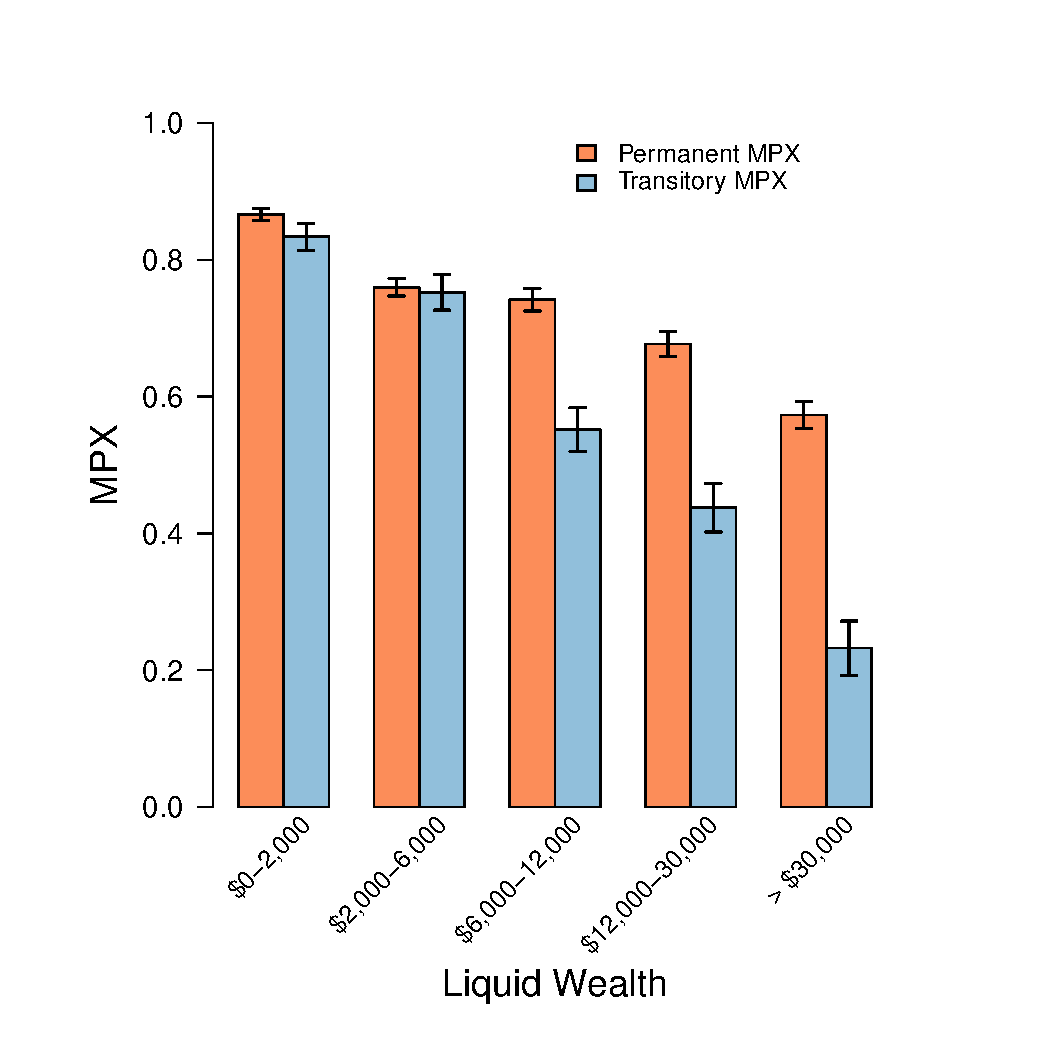
\includegraphics[scale=0.5, trim=1.3cm 0 0 1.3cm]{../Figures/MPXByLiquidWealth_level_lincome_head_CFPBslides.pdf}
}
\section{Monetary Policy}
\frame{
	\frametitle{Monetary Policy: Interest Rate Exposure Channel}
	Some households pay interest \\
	Some households receive interest \\ \pause
	\bigskip
	Monetary policy redistributes between these groups \\
	The aggregate effect depends on differences in spending response \\ \pause
	\bigskip
	Need to know the distribution of MPX by \textbf{Unhedged Interest Rate Exposure}:
	\begin{align*}
	URE_i = Y_i - C_i + A_i - L_i
	\end{align*}
	Where
	\begin{itemize}
		\item $Y_i = $ Total after tax income 
		\item $C_i = $ Total Expenditure, including interest payments
		\item $A_i = $ Maturing assets
		\item $L_i = $ Maturing liabilities
	\end{itemize}
}
\frame{
	\frametitle{MPX by Unhedged Interest Rate Exposure}
		\begin{center}
		\begin{tikzpicture}
		\node (img2) {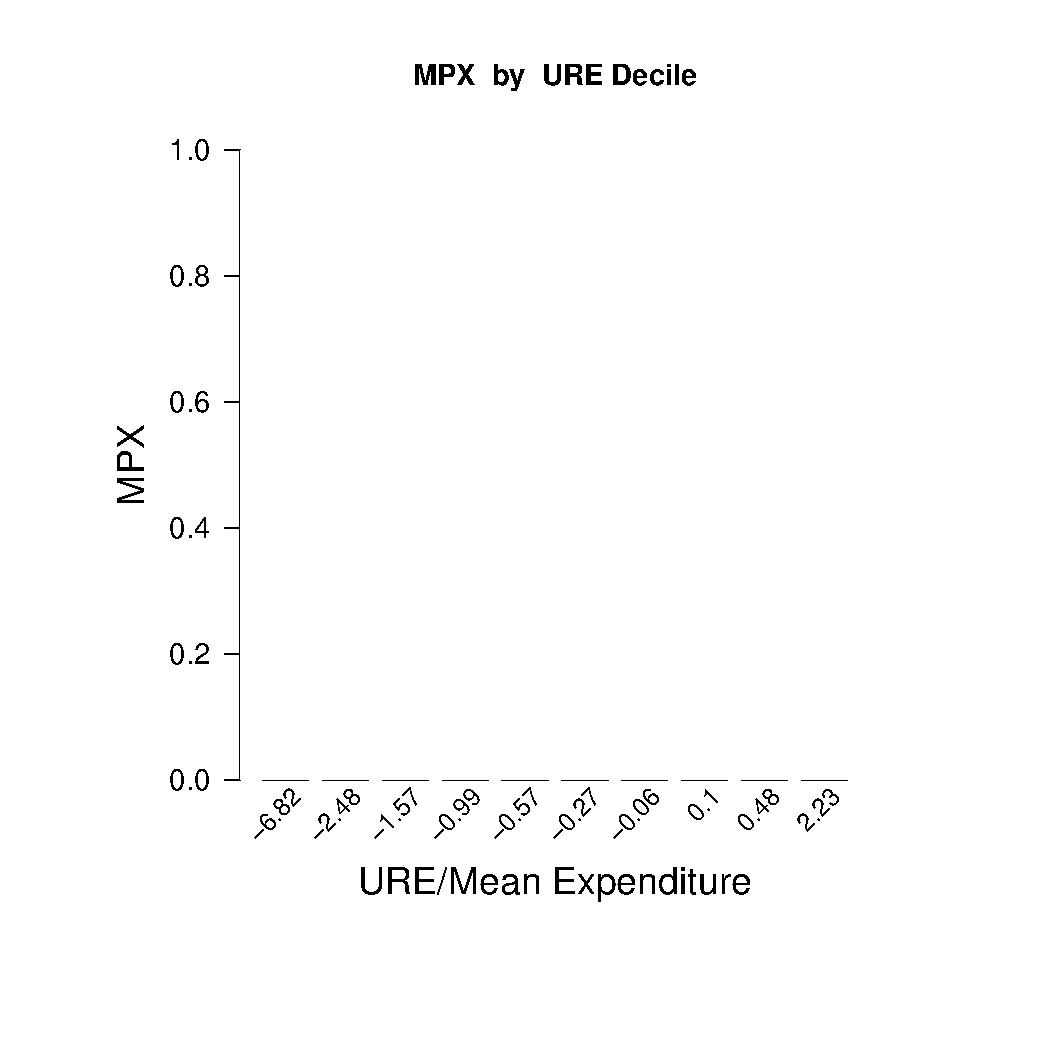
\includegraphics[scale=0.53,trim=0 0 0 1.7cm ,clip]{../Figures/MPXByUREdetailsblank_level_lincome_head.pdf}};
		\node (img3)
		{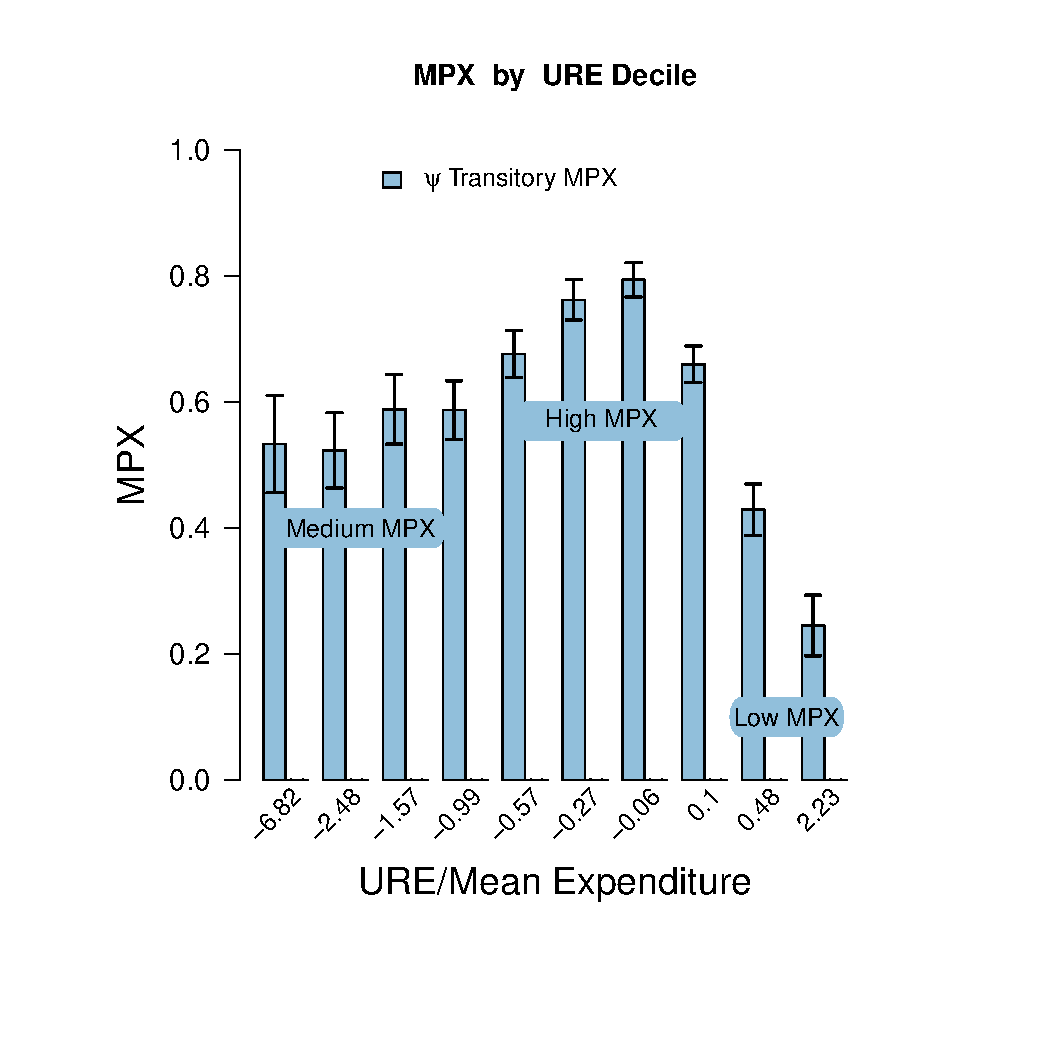
\includegraphics[scale=0.53,trim=0 0 0 1.7cm ,clip]{../Figures/MPXByUREdetails1a_level_lincome_head.pdf}};
		\pause
		\node (img6) {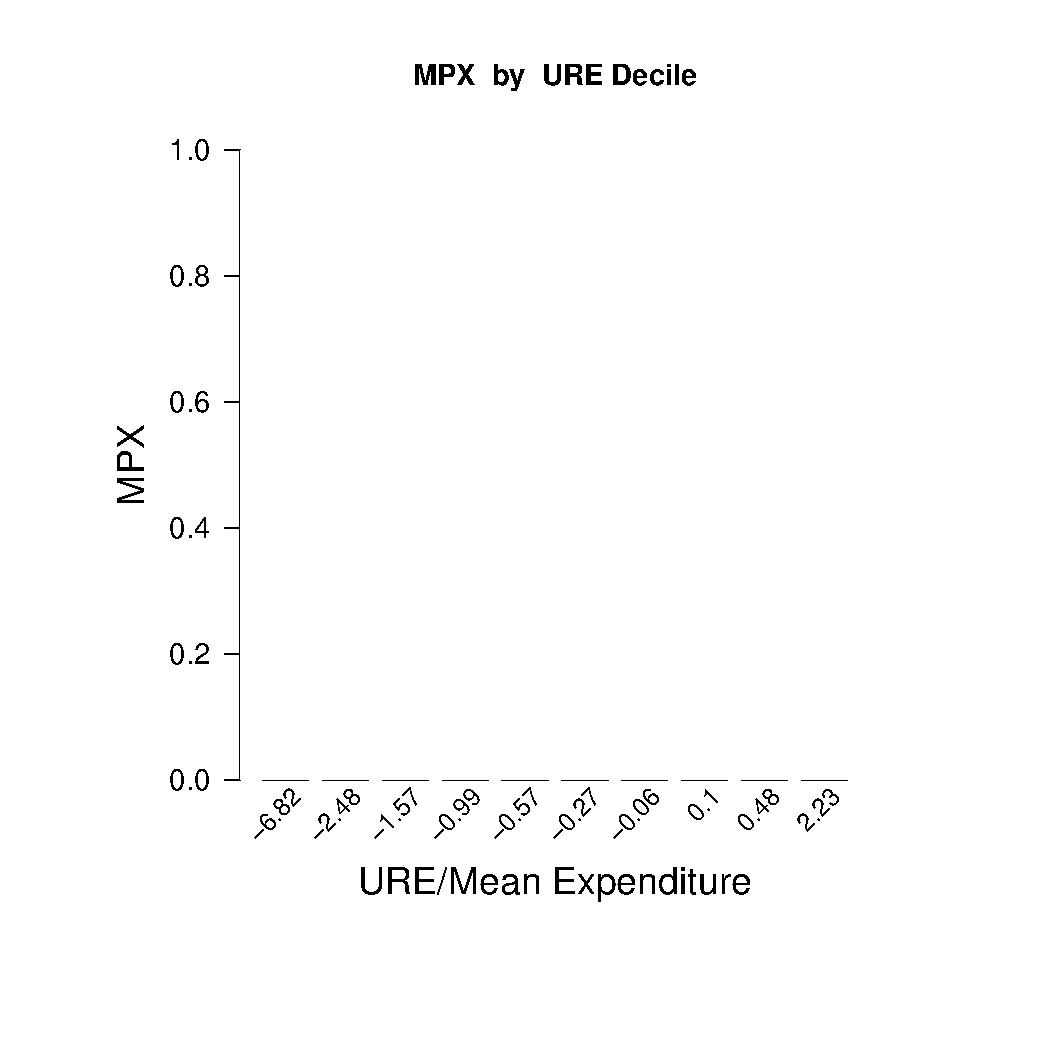
\includegraphics[scale=0.53,trim=0 0 0 1.7cm ,clip]{../Figures/MPXByUREdetailsblank_level_lincome_head.pdf}};
		\node (img7)
		{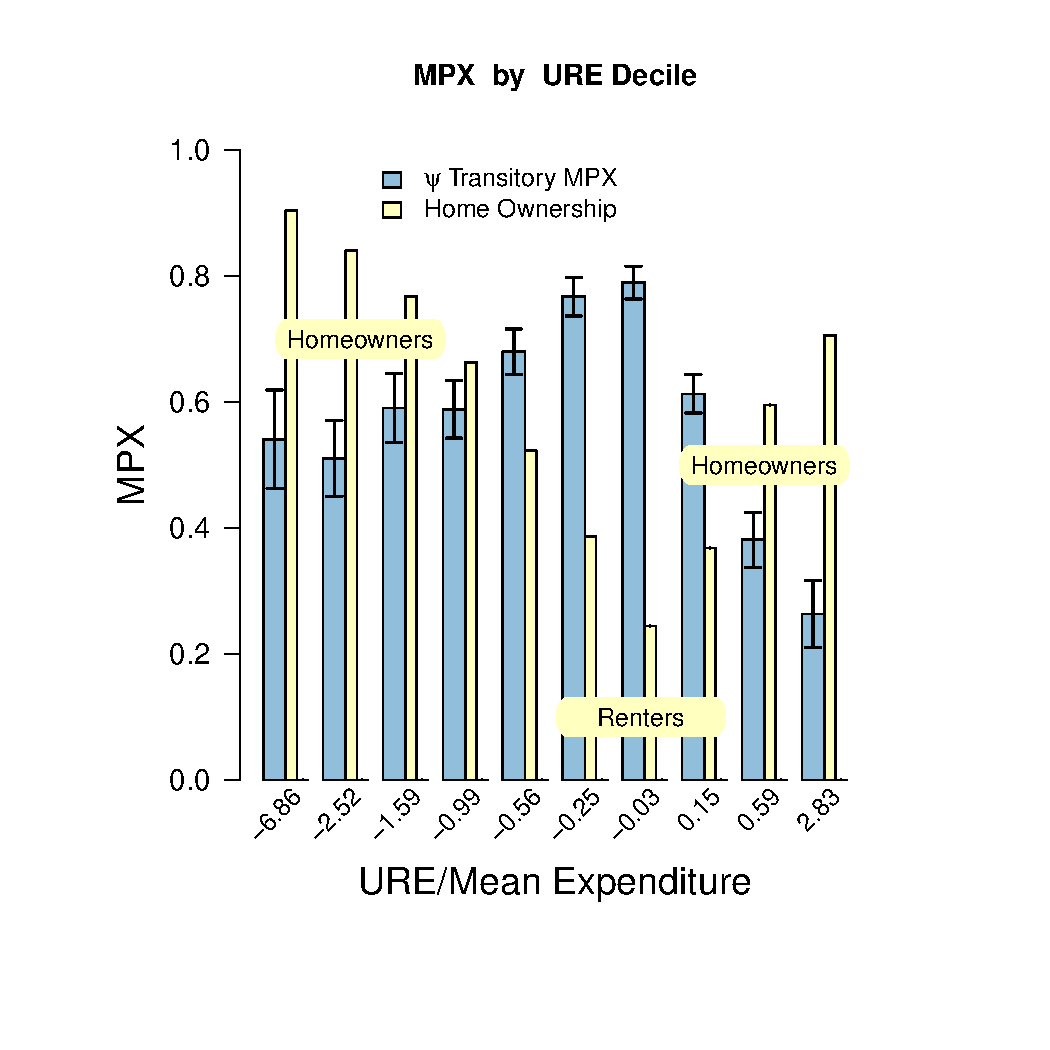
\includegraphics[scale=0.53,trim=0 0 0 1.7cm ,clip]{../Figures/MPXByUREdetails2a_level_lincome_head.pdf}};
		\pause
		\node (img10) {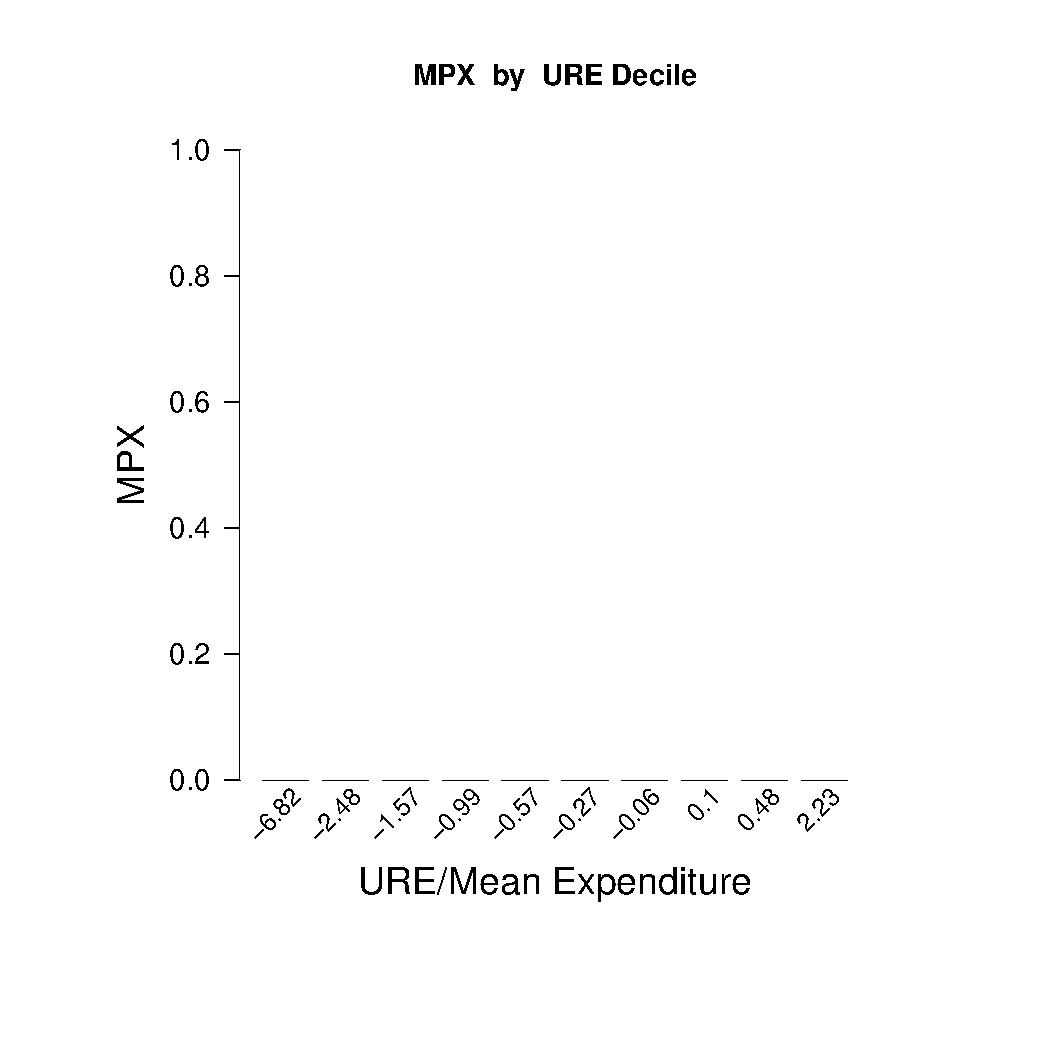
\includegraphics[scale=0.53,trim=0 0 0 1.7cm ,clip]{../Figures/MPXByUREdetailsblank_level_lincome_head.pdf}};
		\node (img11) {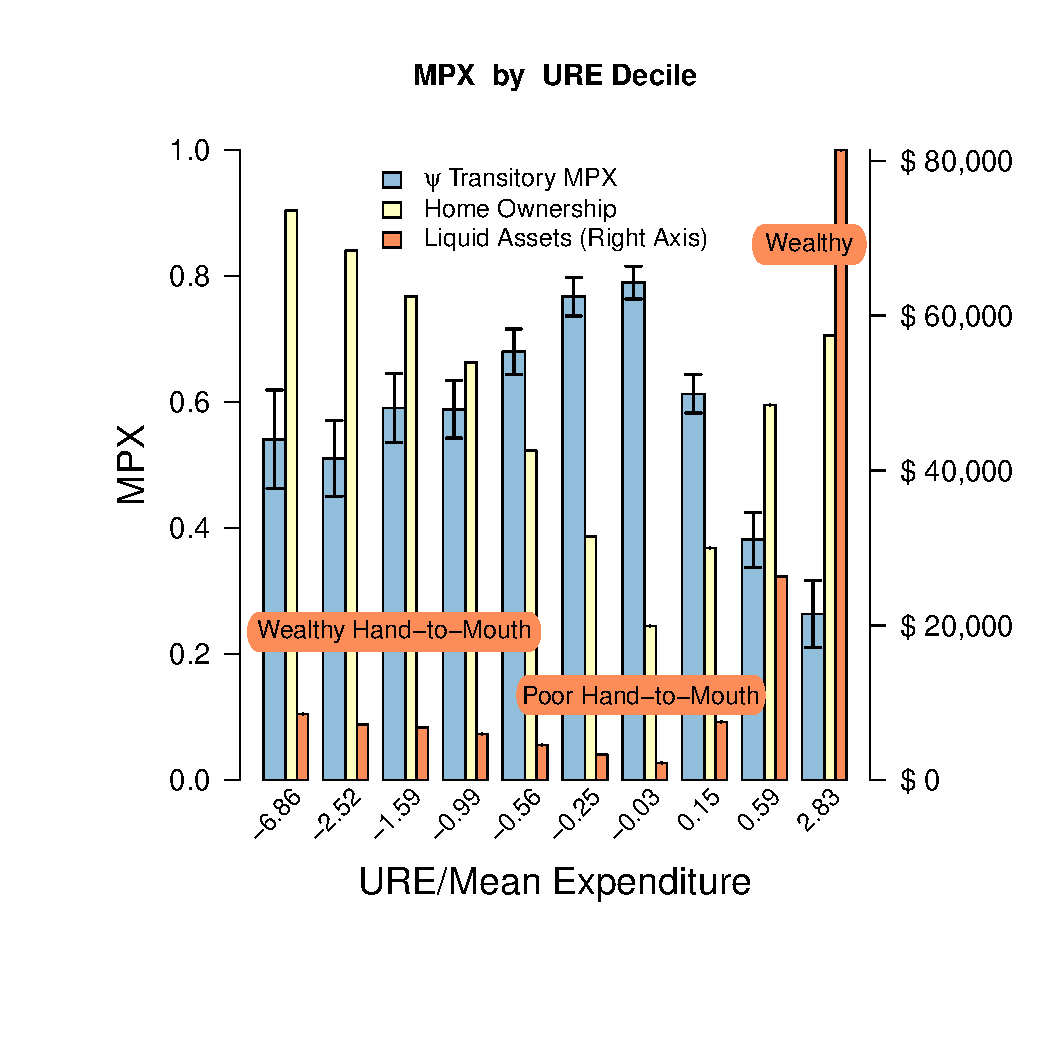
\includegraphics[scale=0.53,trim=0 0 0 1.7cm ,clip]{../Figures/MPXByUREdetails3a_level_lincome_head.pdf}};
		\onslide<1->
		\end{tikzpicture}
	\end{center}
}
\frame{
	\frametitle{Monetary Policy: Interest Rate Exposure Channel}
		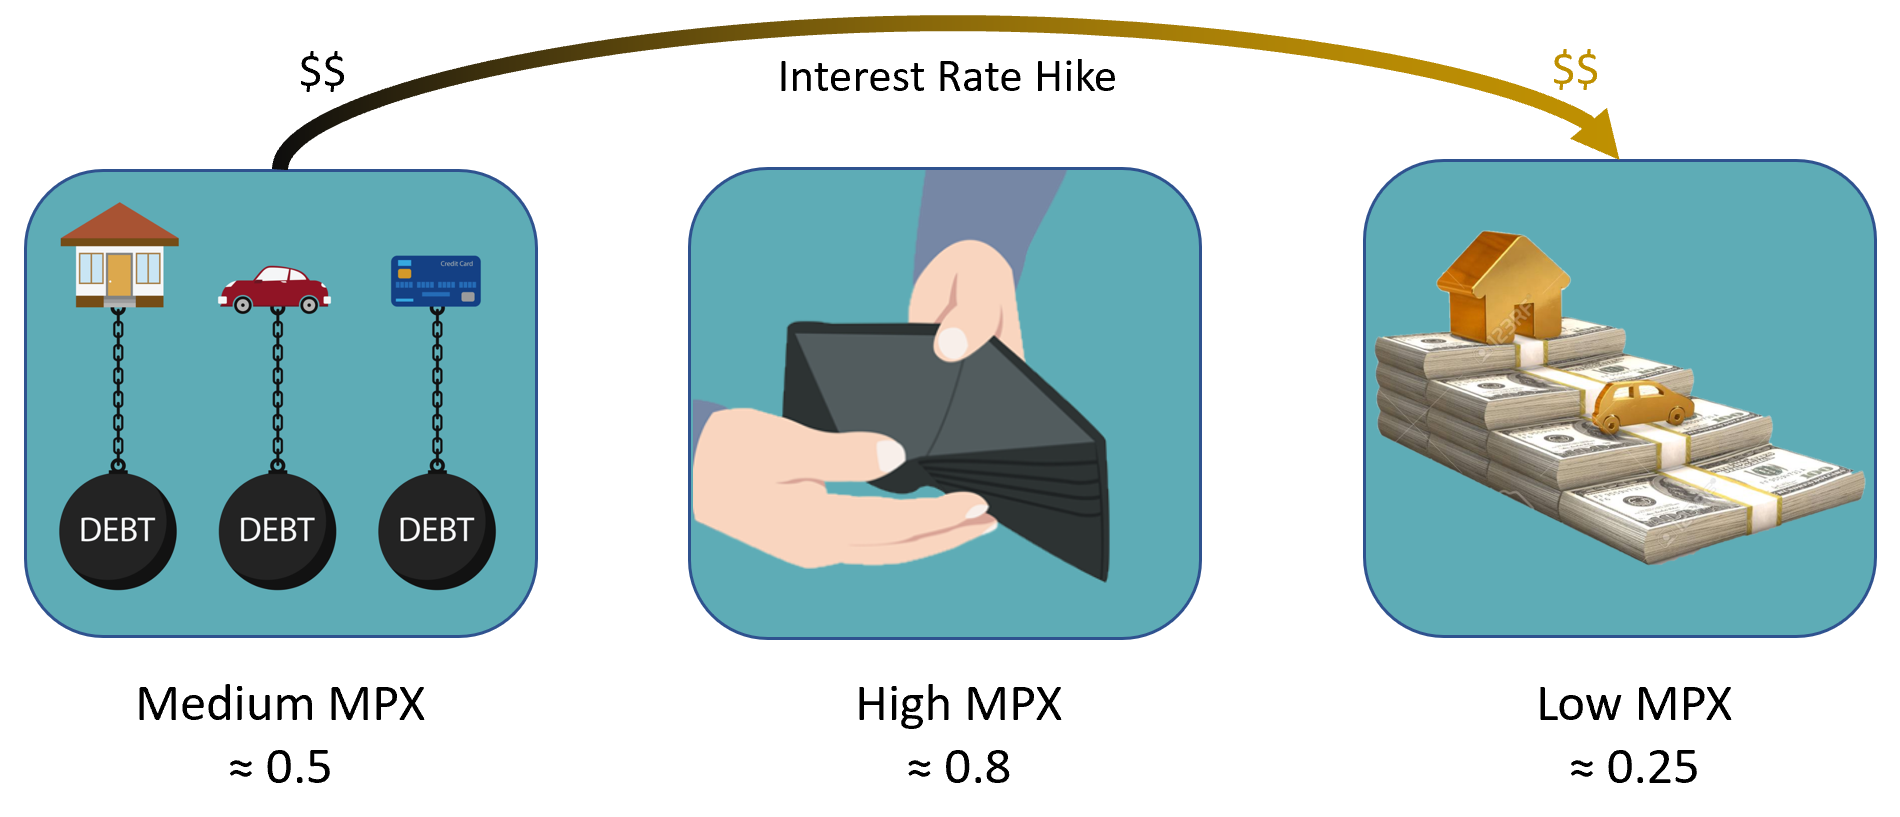
\includegraphics[width=11cm]{./SlideFigures/IRE_Big3.png} \tikz[baseline]{\node(ire){}}
		\vspace{-.5cm}
		\begin{align*}
		\text{1yr rate }&\uparrow \ 1\% \\
		\tikz[baseline]{\node(aggregate){}} \textit{Aggregate}\text{ Spending }&\downarrow \ 26 \text{ basis points}
		\end{align*}
		\begin{tikzpicture}[remember picture,overlay]
		\node (aggregatea)  at ([shift={(1.5,-0.1)}]aggregate) {};
		\node (aggregateb)  at ([shift={(-0.4,-0.4)}]aggregatea) {};
		\draw[blue,thick,->] (aggregatea)  to [in=45,out=225] (aggregateb) node[anchor=north,text = blue] {Through this redistribution channel \textit{alone}};
		\end{tikzpicture}
}
\section{Conclusion}
\frame{
	\frametitle{Conclusion}
	New Method to Estimate Consumption Behavior
	\begin{itemize}
		\item Corrects for Time Aggregation Bias
		\item Estimates align with natural experiment literature
		\item Potential to use on a wide variety of datasets and applications
	\end{itemize}
	\bigskip
	Applied to Danish Registry Data
	\begin{itemize}
	\item Sample Size $\implies$ Sharp Focus on Heterogeneity
	\item High MPX from transitory shocks, Low MPX from Permanent shocks
	\item Quantify Monetary Policy Transmission Channels
\end{itemize}
	\bigskip
	Thank you!
}

\end{document}


